\documentclass{beamer}


% Beamer settings
\usecolortheme{rose}
\beamertemplatenavigationsymbolsempty
\setbeamertemplate{footline}[frame number]

\titlegraphic{%

\includegraphics[height=1cm]{logo-full-colour.png}}

\addtobeamertemplate{frametitle}{}{%
\begin{tikzpicture}[remember picture,overlay]
\node[anchor=north east,yshift=2pt] at (current page.north east) {
\includegraphics[height=1cm]{logo-full-colour.png}};
\end{tikzpicture}}

% Packages
\usepackage{amsmath}

\usepackage{tikz}
\usetikzlibrary{positioning}
\usetikzlibrary{fit}

\usepackage{pgfplots}
\usepgfplotslibrary{fillbetween}

\usepackage{minted}
\usepackage[T1]{fontenc} % Required by minted to ensure dollar signs are produced instead of pound (sterling) signs

\usepackage{multicol}

\usepackage{booktabs}

\usepackage{adjustbox}

% Author
\author{Simon McIntosh-Smith \& Tom Deakin\\University of Bristol}

\date{}



\title{OpenMP for Computational Scientists}

\begin{document}

\frame{\titlepage}

%-------------------------------------------------------------------------------
\begin{frame}
\frametitle{Thanks}
Thanks go to the following authors, whose own OpenMP tutorials have inspired this one:
\begin{itemize}
  \item Tim Mattson (Intel)
  \item Simon McIntosh-Smith and the HPC team (UoBristol)
  \item Gethin Williams (UoBristol)
  \item and many others
\end{itemize}
\end{frame}

%-------------------------------------------------------------------------------
\begin{frame}
\frametitle{Exercises}
\begin{itemize}
\item This is a hands-on course!
\item Exercises will be set for you to try programming OpenMP yourselves.
\item Sample solutions also provided.
\item All the exercises will be in Fortran.
\end{itemize}

Download code (and slides) from:
\url{https://github.com/UoB-HPC/openmp-for-cs}
\end{frame}

%-------------------------------------------------------------------------------
\section{Outline}
\begin{frame}
\frametitle{Course Outline}
Organised as 6 sessions teaching OpenMP plus top-tips for getting good performance.
\begin{enumerate}
  \item OpenMP overview
  \item Data sharing and reductions
  \item Code optimisations
  \item Vectoriation, NUMA and MPI interop
  \item GPU programming with OpenMP
  \item Tasks and Tools
\end{enumerate}
\end{frame}
%-------------------------------------------------------------------------------

\begin{frame}
\frametitle{The first exercise}
\begin{itemize}
  \item At the end of this session, you will be able to parallelise a (simple) 5-point stencil code using OpenMP!
  \item The other sessions provide you with details you might need for real world codes.
\end{itemize}
\end{frame}

%-------------------------------------------------------------------------------
\begin{frame}
\frametitle{What is OpenMP?}

A collection of compiler directives, library routines, and environment variables for parallelism for shared memory parallel programs.

\begin{itemize}
  \item Create and manage parallel programs while permitting portability.
  \item User-directed parallelization.
\end{itemize}

A \emph{specfication} of annotations you can make to your program in order to make it parallel.

\end{frame}

%-------------------------------------------------------------------------------
\begin{frame}[fragile]
\frametitle{Syntax}
\begin{itemize}
\item OpenMP mostly formed of \emph{compiler directives}\\
  \begin{minted}{fortran}
  !$omp construct [clause [clause]...]
  \end{minted}
  These tell the compiler to insert some extra code on your behalf.

\item Compiler directives usually apply to a \emph{structured block} of statements.
Limited scoping in Fortran means often need \emph{end} directives.
  \begin{minted}{fortran}
  !$omp construct
  ... ! lines of Fortran code
  !$omp end construct
  \end{minted}

\item Library API calls
  \begin{minted}{fortran}
  use omp_lib
  call omp_...()
  \end{minted}

\end{itemize}
\end{frame}

%-------------------------------------------------------------------------------
\begin{frame}[fragile]
\frametitle{Building with OpenMP}

Turn on OpenMP in the compiler:
\begin{minted}{bash}
gfortran *.f90 -fopenmp # GNU
ifort *.f90 -qopenmp    # Intel
ftn *.f90               # Cray (on by default)
pgf90 *.f90 -mp         # PGI
\end{minted}

To also use the API calls within the code, use the library:
\begin{minted}{fortran}
USE omp_lib
\end{minted}

\begin{alertblock}{Note}
No need to include the library if only using the compiler directives.
The library only gets you the API calls.
\end{alertblock}
\end{frame}

%-------------------------------------------------------------------------------
\begin{frame}
\frametitle{Shared memory}
OpenMP is for shared memory programming: all threads have access to a shared address space.

A typical HPC node consisting of 2 multi-core CPUs.
\begin{center}
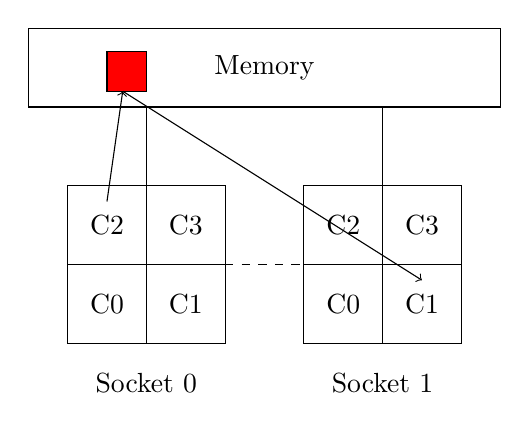
\begin{tikzpicture}
  % Draw 4 cores for socket 0
  \draw (0,0) rectangle (1,1);
  \draw (0.5,0.5) node {C0};
  \draw (1,0) rectangle (2,1);
  \draw (1.5,0.5) node {C1};
  \draw (0,1) rectangle (1,2);
  \draw (0.5,1.5) node {C2};
  \draw (1,1) rectangle (2,2);
  \draw (1.5,1.5) node {C3};
  \draw (1,-0.5) node {Socket 0};

  % Draw 4 cores for socket 1
  \draw (3,0) rectangle (4,1);
  \draw (3.5,0.5) node {C0};
  \draw (4,0) rectangle (5,1);
  \draw (4.5,0.5) node {C1};
  \draw (3,1) rectangle (4,2);
  \draw (3.5,1.5) node {C2};
  \draw (4,1) rectangle (5,2);
  \draw (4.5,1.5) node {C3};
  \draw (4,-0.5) node {Socket 1};

  % Draw large memory
  \draw (-0.5,3) rectangle (5.5,4);
  \draw (2.5,3.5) node {Memory};

  % Connect sockets to memory
  \draw (1,2) -- (1,3);
  \draw (4,2) -- (4,3);
  \draw[dashed] (2,1) -- (3,1); % QPI

  % Show memory shared
  \pause
  \draw[fill=red] (0.5,3.2) rectangle (1,3.7);
  \draw[->] (0.5,1.8) -- (0.7,3.2);
  \draw[->] (0.7,3.2) -- (4.5,0.8);

\end{tikzpicture}
\end{center}
\emph{All} threads (running on a core) access the same memory.

Different to MPI, where processes cannot see memory of another without explicit communication.

\end{frame}

%-------------------------------------------------------------------------------
\begin{frame}
\frametitle{Fork-join model}
Serial/sequential execution:
\begin{center}
\begin{tikzpicture}
  \draw[->] (0,0) -- (8,0);
\end{tikzpicture}
\end{center}

In a \emph{fork-join} model, code starts serial, \emph{forks} a \emph{team} of threads then \emph{joins} them back to serial execution.
\begin{center}
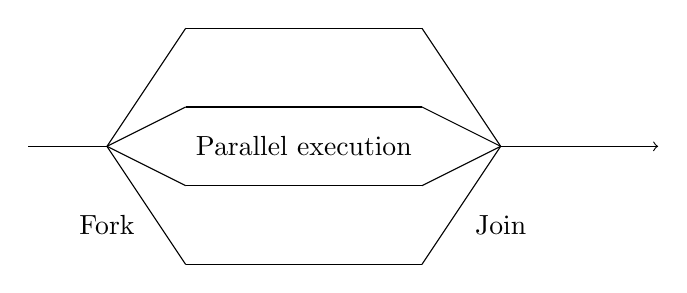
\begin{tikzpicture}
  \draw (0,0) -- (1,0);

  % Fork
  \draw (1,0) -- (2,1.5);
  \draw (1,0) -- (2,0.5);
  \draw (1,0) -- (2,-0.5);
  \draw (1,0) -- (2,-1.5);
  \draw (1,-1) node {Fork};

  % Run in parallel
  \draw (2,1.5)  -- (5,1.5);
  \draw (2,0.5)  -- (5,0.5);
  \draw (2,-0.5) -- (5,-0.5);
  \draw (2,-1.5) -- (5,-1.5);
  \draw (3.5,0) node {Parallel execution};

  % Join
  \draw (5,1.5)  -- (6,0);
  \draw (5,0.5)  -- (6,0);
  \draw (5,-0.5) -- (6,0);
  \draw (5,-1.5) -- (6,0);
  \draw (6,-1) node {Join};

  % Serial end
  \draw[->] (6,0) -- (8,0);
\end{tikzpicture}
\end{center}

Nested threads are allowed, where a thread forks it's own team of threads.
\end{frame}

%-------------------------------------------------------------------------------
\begin{frame}[fragile]
\frametitle{Creating OpenMP threads}
\begin{minted}{fortran}
program hello

!$omp parallel
  print *, "Hello"
!$omp end parallel

end program hello
\end{minted}

Threads \emph{redundantly} execute code in the block.

Each thread will output \mintinline{bash}|Hello|.

Threads are synchronised at the end of the parallel region.

\end{frame}

%-------------------------------------------------------------------------------
\begin{frame}[fragile]
\frametitle{Pthreads}

\begin{minted}[fontsize=\small]{fortran}
program hello
  use fpthread
  intger :: i, err
  integer :: N = 4
  type(fpthread_t) :: tid(N)

  do i = 1, N
    call fpthread_create(tid(i), NULL, run, NULL, err)
  end do
  do i = 1, N
    call fpthread_join(tid(i), NULL, err)
  end do

  subroutine run
    print *, "Hello"
  end subroutine run
end program hello
\end{minted}

\end{frame}

%-------------------------------------------------------------------------------
\begin{frame}
\frametitle{OpenMP and Pthreads}
\begin{itemize}
  \item Pthreads is very error prone and verbose.
  \item The OpenMP \mintinline{fortran}|!$omp parallel| abstracts this away.
  \item The compiler directive inserts this extra code for your behalf.
  \item Pthreads requires wrapping up my parallel work in subroutines.
    \begin{itemize}
      \item Kernels are a useful abstraction used in many programming models.
    \end{itemize}
  \item OpenMP much more convenient for \emph{incrementally} adding parallelism to your code.
\end{itemize}
\end{frame}

%-------------------------------------------------------------------------------
\begin{frame}[fragile]
\frametitle{Setting number of threads}
Need to be able to set the number of threads to launch.

OpenMP has 3 ways to do this:
\begin{itemize}
  \item Environment variables
  \begin{minted}{bash}
  OMP_NUM_THREADS=16
  \end{minted}

  \item API calls
  \begin{minted}{fortran}
  call omp_set_num_threads(16)
  \end{minted}

  \item Clauses
  \begin{minted}{fortran}
  !$omp parallel num_threads(16)
  !$omp end parallel
  \end{minted}
\end{itemize}

In general it's better to use environment variables to set this as gives you more flexibility at runtime.
\end{frame}

%-------------------------------------------------------------------------------
\begin{frame}[fragile]
\frametitle{Thread API calls}
Most parallel programs are written in a SPMD style: {\bf S}ingle {\bf P}rogram, {\bf M}ultiple {\bf D}ata.
\begin{itemize}
  \item MPI has a SPMD model.
  \item Threads run the same code, and use their ID to work out which data to operate on.
\end{itemize}

The OpenMP API gives you calls to determine thread information when \emph{inside} a parallel region:
\begin{itemize}
  \item Get number of threads
    \begin{minted}{fortran}
    nthreads = omp_get_num_threads()
    \end{minted}

  \item Get thread ID
    \begin{minted}{fortran}
    tid = omp_get_thread_num()
    \end{minted}

\end{itemize}
\end{frame}

%-------------------------------------------------------------------------------
\begin{frame}[fragile]
\frametitle{Vector add}
Walkthrough parallelising vector addition using OpenMP.

\begin{minted}[fontsize=\small,linenos]{fortran}
program vecadd
  integer :: N = 1024  ! Length of array
  ! Arrays
  real(kind=8), allocatable, dimension(:) :: A, B, C
  integer :: i         ! Loop counter

  ! Allocate and initilise vectors
  allocate(A(N), B(N), C(N))
  A = 1.0; B = 2.0; C = 0.0

  ! Vector add
  do i = 1, N
    C(i) = A(i) + B(i)
  end do

  deallocate(A,B,C)
end program vecadd
\end{minted}
\end{frame}

%-------------------------------------------------------------------------------
\begin{frame}[fragile]
\frametitle{Vector add: Step 1}
Add parallel region around work
\begin{minted}{fortran}
  !$omp parallel
  do i = 1, N
    C(i) = A(i) + B(i)
  end do
  !$omp end parallel
\end{minted}
Every thread will now do the entire vector addition --- redundantly!
\end{frame}

%-------------------------------------------------------------------------------
\begin{frame}[fragile]
\frametitle{Vector add: Step 2}
Get thread IDs
\begin{minted}{fortran}
  integer :: tid, nthreads

  !$omp parallel
  tid = omp_get_thread_num()
  nthreads = omp_get_num_threads()

  do i = 1, N
    C(i) = A(i) + B(i)
  end do
  !$omp end parallel
\end{minted}

\pause
\begin{alertblock}{Incorrect behaviour at runtime}
What's the problem here?
\end{alertblock}
\end{frame}

%-------------------------------------------------------------------------------
\begin{frame}[fragile]
\frametitle{Vector add: Step 2, take 2}

\begin{itemize}
  \item In OpenMP, all variables are \emph{shared} between threads.
  \item But each thread needs own copy of \mintinline{fortran}|tid|.
  \item Solution: use the \mintinline{fortran}|private| clause on the \mintinline{fortran}|parallel| region.
  \item This gives each thread it's own unique copy in memory for the variable.
\end{itemize}

\begin{minted}{fortran}
  integer :: tid, nthreads

  !$omp parallel private(tid)
  tid = omp_get_thread_num()
  nthreads = omp_get_num_threads()

  do i = 1, N
    C(i) = A(i) + B(i)
  end do
  !$omp end parallel
\end{minted}
Much more information about data sharing clausing in next session.
\end{frame}

%-------------------------------------------------------------------------------
\begin{frame}[fragile]
\frametitle{Vector add: Step 3}
Finally, share the iteration space between the threads.
\begin{minted}{fortran}
  integer :: tid, nthreads

  !$omp parallel private(tid)
  tid = omp_get_thread_num()
  nthreads = omp_get_num_threads()

  do i = 1+(tid*N/nthreads), (tid+1)*N/nthreads
    C(i) = A(i) + B(i)
  end do
  !$omp end parallel
\end{minted}
\begin{block}{Remember}
Thread IDs are numbered from 0 in OpenMP.
Be careful with your index calculation.
\end{block}
\end{frame}

%-------------------------------------------------------------------------------
\begin{frame}[fragile]
\frametitle{Worksharing}

\begin{itemize}
\item The SPMD approach requires lots of bookkeeping.
\item Common pattern of splitting loop iterations between threads.
\item OpenMP has worksharing constructs to help with this.
\item Used within a parallel region.
\item Loop iterator is made \mintinline{fortran}|private| by default.
\end{itemize}

\begin{minted}{fortran}
  !$omp parallel
  !$omp do
  do i = 1, N
    C(i) = A(i) + B(i)
  end do
  !$omp end do
  !$omp end parallel
\end{minted}


Generally it's convenient to combine the directives:
\begin{minted}{fortran}
!$omp parallel do
!$omp end parallel do
\end{minted}

\end{frame}

%-------------------------------------------------------------------------------
\begin{frame}
\frametitle{Synchronisation}
Just introduce this stuff.
Critical, atomic, barier, ordered, flush, locks
\end{frame}

%-------------------------------------------------------------------------------
\begin{frame}
\frametitle{Scheduling}
schedule clause

\end{frame}

%-------------------------------------------------------------------------------
\begin{frame}
\frametitle{Nested loops}
Collapse
Mention issues with SIMD/alignment?

\end{frame}

%-------------------------------------------------------------------------------
\begin{frame}
\frametitle{5-point stencil example}
Do parallelism of a structured grid 5-point stencil
\end{frame}

%-------------------------------------------------------------------------------
\begin{frame}
\frametitle{nowait clause}
nowait
\end{frame}

%-------------------------------------------------------------------------------
\begin{frame}
\frametitle{Sections}
sections, single, tasks?
\end{frame}

%-------------------------------------------------------------------------------
\begin{frame}
\frametitle{Nested threads}
sections, single, tasks?
\end{frame}

%-------------------------------------------------------------------------------
\begin{frame}
\frametitle{Resources}
OpenMP secficiation (not for the faint hearted)
Online tutorials
Books
\end{frame}

%-------------------------------------------------------------------------------

\end{document}
